% =====================================================================
% Sección: Integración del modelo del pedal con CARLA
% Para AEB_IEEE (IEEEtran) en Overleaf. Solo necesita graphicx.
% Las imágenes pueden estar en la carpeta figuras_pedal/ o sueltas junto
% al archivo principal: las dos rutas funcionan.
% =====================================================================
\begingroup
\graphicspath{{figuras_pedal/}{./}}
\section{Integración del modelo del pedal con CARLA}
\label{sec:pedal_carla}

El actuador idealizado de CARLA se reemplazó por un modelo en Python del
actuador Nanotec LGA561 con el controlador C5-E, construido a partir de la
calibración proporcionada por Bloom Drive. El modelo se ejecuta dentro del
lazo de simulación de 20~Hz, de modo que el freno que recibe el vehículo
incluye el retardo y los límites del mecanismo. La lógica de decisión del
AEB no se modificó. El modelo es solo de simulación: no se conecta al
hardware.

\subsection{Cadena de integración}

La Fig.~\ref{fig:pedal_cadena} muestra la cadena que se ejecuta en cada
ciclo de 0.05~s. La demanda $u_b$ del AEB entra al modelo del controlador en
modo \textit{Profile Position} (6060h${}=1$), que la convierte en la
referencia $z_{ref}=0.2\,u_b$~mm (6900~ticks equivalen a 20~mm). Un
generador de perfil trapezoidal mueve la varilla con velocidad máxima de
30~mm/s. La posición $z$ fija el giro del pedal $\theta_p$ por la geometría
del contacto, a 110~mm del pivote, y el freno logrado es
\begin{equation}
  p_{log} = 100\,\mathrm{clip}\left(\frac{\theta_p-\theta_j}
            {\theta_{p,\max}-\theta_j},\,0,\,1\right),
  \label{eq:pedal_plog}
\end{equation}
donde $\theta_j$ es el juego del freno y $\theta_{p,\max}$ el giro con la
varilla a 20~mm (Tabla~\ref{tab:pedal_param}). Una primera versión del
modelo, en modo \textit{Profile Torque}, limitaba el freno a 92.6~\%; el
modo de posición alcanza el 100~\%. En cada ciclo, el modelo envía su estado
por UDP a un visualizador del pedal y agrega al registro del ensayo el avance
de la varilla, el ángulo, la fuerza y la corriente estimadas.

\begin{figure}[!t]
  \centering
  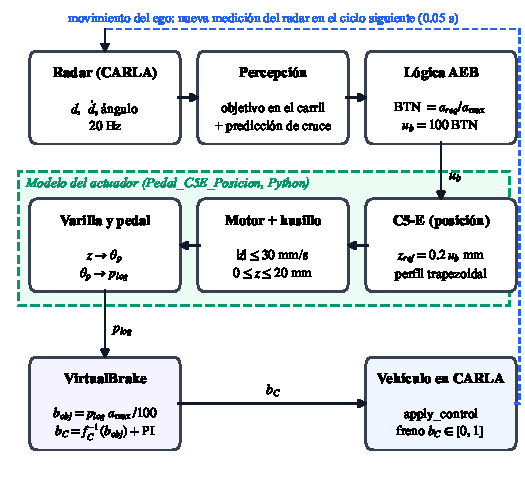
\includegraphics[width=\columnwidth]{fig_cadena.pdf}
  \caption{Cadena de frenado con el modelo del pedal. La demanda $u_b$ pasa
  por el modelo del actuador antes de llegar a CARLA; el lazo se cierra a
  través del movimiento del vehículo y del radar.}
  \label{fig:pedal_cadena}
\end{figure}

\subsection{Traducción al freno de CARLA}

CARLA recibe un freno adimensional $b_C\in[0,1]$ cuya desaceleración no es
lineal y llega a 8.68~m/s$^2$, por encima de $a_{\max}=6.8$~m/s$^2$ del
Porsche. Por ello, el freno logrado se convierte en una desaceleración
objetivo y después en $b_C$ con el mapa medido $f_C$
(Tabla~\ref{tab:pedal_param}) y una corrección PI con la desaceleración
medida $b_{med}$:
\begin{equation}
  b_{obj} = \frac{p_{log}}{100}\,a_{\max},
  \label{eq:pedal_bobj}
\end{equation}
\begin{equation}
  b_C = \mathrm{clip}\left(f_C^{-1}(b_{obj}) + k_p e + k_i \int e\,dt,\ 0,\ 1\right),
  \label{eq:pedal_bc}
\end{equation}
con $e=b_{obj}-b_{med}$.
Si $b_{med}$ supera $a_{\max}$, en el ciclo siguiente $b_C$ se escala por
$a_{\max}/b_{med}$.

\begin{table}[!t]
  \caption{Parámetros de la cadena pedal--CARLA}
  \label{tab:pedal_param}
  \centering
  \footnotesize
  \begin{tabular}{@{}ll@{}}
    \hline
    Parámetro & Valor \\
    \hline
    Modo del C5-E & \textit{Profile Position} (6060h${}=1$) \\
    Escala de la referencia & 6900 ticks $\leftrightarrow$ 20 mm \\
    Velocidad máxima de perfil & 30 mm/s$^{a}$ \\
    Aceleración / desaceleración de perfil & 120 / 180 mm/s$^2$ $^{b}$ \\
    Juego del freno $\theta_j$ & 0.7$^\circ$ $^{b}$ \\
    Giro con la varilla a 20 mm, $\theta_{p,\max}$ & 9.7$^\circ$ \\
    Mapa $f_C$: $b_C=0.2/0.4/0.6/0.8/1.0$ & 3.66/5.55/6.67/7.69/8.68 m/s$^2$ \\
    Ganancias PI $k_p$ / $k_i$ & 0.05 / 0.8 \\
    \hline
    \multicolumn{2}{@{}l@{}}{\scriptsize $^{a}$Catálogo a 24 V. $^{b}$Supuesto de modelado, sin medir.}
  \end{tabular}
\end{table}

\subsection{Resultados en CARLA}

La Tabla~\ref{tab:pedal_resultados} resume siete corridas con el modelo del
pedal. Seis terminaron sin contacto, con separaciones finales de 1.31 a
2.34~m. En todas, el pedal empezó a frenar 0.20~s después de la demanda,
llegó a 25~\% a los 0.35~s y a 50~\% a los 0.50~s, dentro del tiempo de
respuesta de 0.4--0.6~s reportado por Bloom Drive. En
\texttt{MI\_ESCENARIO\_40KMH\_PEATON}, el pedal tardó 1.35~s en llegar a
50~\% porque la demanda se mantuvo cerca de ese valor.

\begin{table}[!t]
  \caption{Resultados en CARLA con el modelo del pedal}
  \label{tab:pedal_resultados}
  \centering
  \footnotesize
  \setlength{\tabcolsep}{4pt}
  \begin{tabular}{@{}lcccc@{}}
    \hline
    Ensayo & $v_0$ & $u_b$ inicial; $d$ & $t_{50}$ & Resultado \\
           & [km/h] & [\%; m] & [s] & \\
    \hline
    PROPIO\_FRENA\_18\_3453$^{\dagger}$ & 18 & 56; 6.1  & 0.50 & 2.34 m \\
    ENCAP\_CCRb\_6\_12                   & 50 & 62; 12.1 & 0.50 & 1.31 m \\
    ENCAP\_CCRb\_6\_12$^{\dagger}$       & 50 & 62; 12.1 & 0.50 & 2.34 m \\
    Peatón 30 km/h                       & 30 & 53; 13.2 & 0.55 & 1.58 m \\
    Niño tarde, con predicción           & 30 & 54; 13.2 & 0.55 & 1.59 m \\
    Niño tarde, sin predicción           & 30 & 100; 6.4 & 0.50 & 21.7 km/h$^{\ast}$ \\
    Peatón 40 km/h con líder             & 40 & 52; $\approx$20 & 1.35 & 1.96 m \\
    \hline
    \multicolumn{5}{@{}p{\columnwidth}@{}}{\scriptsize $u_b$ inicial; $d$:
    demanda y distancia al objetivo al activarse el frenado. $t_{50}$: tiempo
    hasta $p_{log}\geq 50$~\%. Resultado: separación final sin contacto.
    $^{\dagger}$Con tráfico de ambiente. $^{\ast}$Velocidad relativa de
    impacto.}
  \end{tabular}
\end{table}

\textit{Escenario Euro NCAP CCRb.} La Fig.~\ref{fig:pedal_encap} muestra la
corrida sin tráfico. El AEB pidió 62~\% a 1.20~s, 0.2~s después de que el
líder frenó; el pedal alcanzó 50~\% a 1.70~s y siguió la demanda con un
retardo de 0.2 a 0.3~s (Fig.~\ref{fig:pedal_encap}a--b). Cerca de 3.5~s la
demanda bajó a 33~\% y volvió a 100~\%; la varilla siguió ese cambio más
lentamente, limitada a 30~mm/s. El ego se detuvo a 4.35~s, a 1.31~m del
líder, con una desaceleración media de 4.2~m/s$^2$ por encima de 7~km/h. La
Fig.~\ref{fig:pedal_fotos}a muestra el instante $t=2.0$~s.

\begin{figure}[!t]
  \centering
  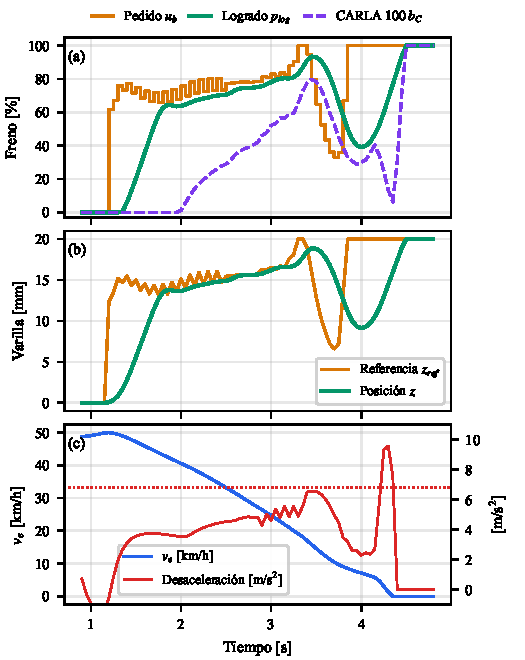
\includegraphics[width=\columnwidth]{fig_encap_cadena.pdf}
  \caption{\texttt{ENCAP\_CCRb\_6\_12} sin tráfico: (a) freno pedido $u_b$,
  logrado $p_{log}$ y enviado a CARLA $b_C$; (b) referencia y posición de la
  varilla; (c) velocidad y desaceleración del ego. La línea punteada marca
  $a_{\max}=6.8$~m/s$^2$.}
  \label{fig:pedal_encap}
\end{figure}

\textit{Peatón que cruza tarde.} En \texttt{MI\_ESCENARIO\_PEATON\_30KMH},
un niño sale entre autos estacionados frente al ego, que va a 30~km/h, y se
detiene en el carril. En el escenario base empieza a cruzar cuando al ego le
faltan 4.2~s para alcanzarlo; en la variante tardía, 3.2~s. En esta
variante, la predicción de cruce lo marcó como amenaza antes de que entrara
al carril, y el AEB pidió
freno a 9.30~s con el niño a 13.2~m (Fig.~\ref{fig:pedal_fotos}b). Sin la
predicción, la demanda llegó a 10.15~s, con el niño ya en el carril a
6.4~m. Aunque pidió 100~\%, el pedal tardó 0.5~s en llegar a la mitad y el
ego atropelló al niño a 21.7~km/h (Fig.~\ref{fig:pedal_fotos}c). La
Fig.~\ref{fig:pedal_nino} compara ambas corridas: frenar 0.85~s antes
equivale a unos 7~m de distancia a 30~km/h.

\begin{figure}[!t]
  \centering
  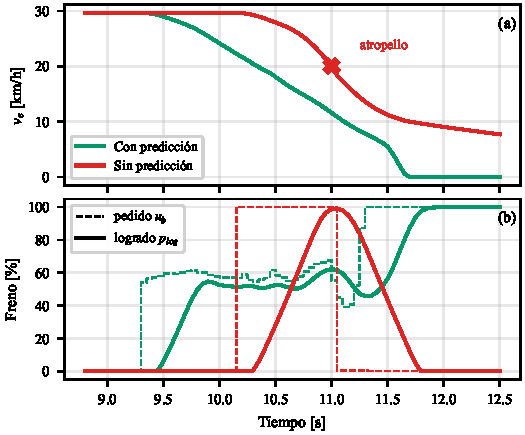
\includegraphics[width=\columnwidth]{fig_nino_tarde.pdf}
  \caption{Niño que cruza tarde, con y sin predicción de cruce: (a) velocidad
  del ego; (b) freno pedido y logrado por el pedal.}
  \label{fig:pedal_nino}
\end{figure}

\begin{figure*}[!t]
  \centering
  \begin{minipage}[t]{0.325\textwidth}
    \centering
    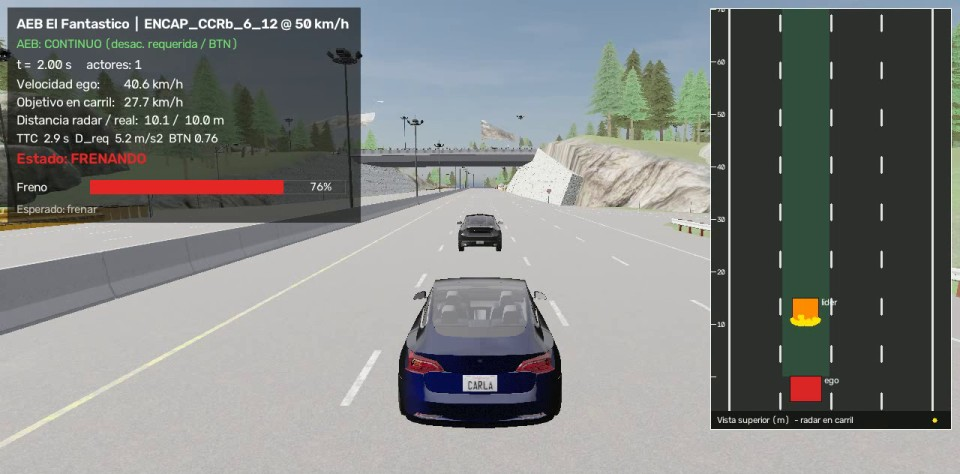
\includegraphics[width=\linewidth]{foto_encap.jpg}\\
    \footnotesize (a)
  \end{minipage}\hfill
  \begin{minipage}[t]{0.325\textwidth}
    \centering
    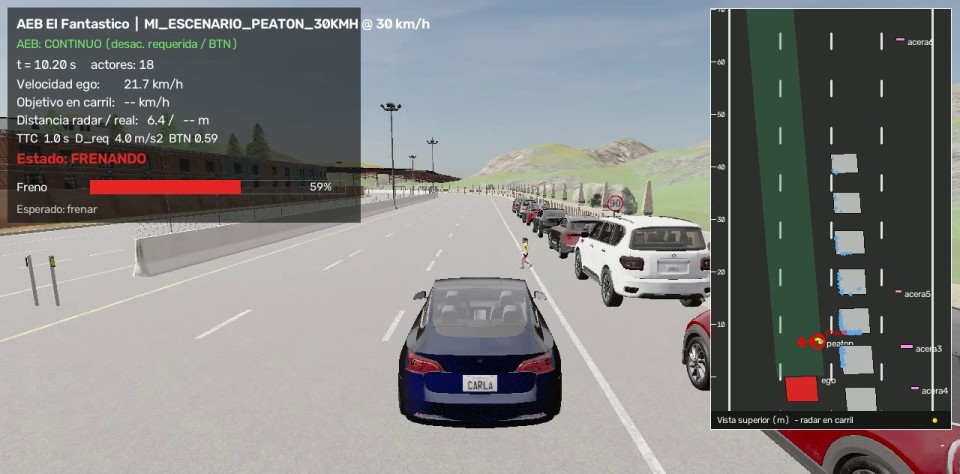
\includegraphics[width=\linewidth]{foto_nino_con.jpg}\\
    \footnotesize (b)
  \end{minipage}\hfill
  \begin{minipage}[t]{0.325\textwidth}
    \centering
    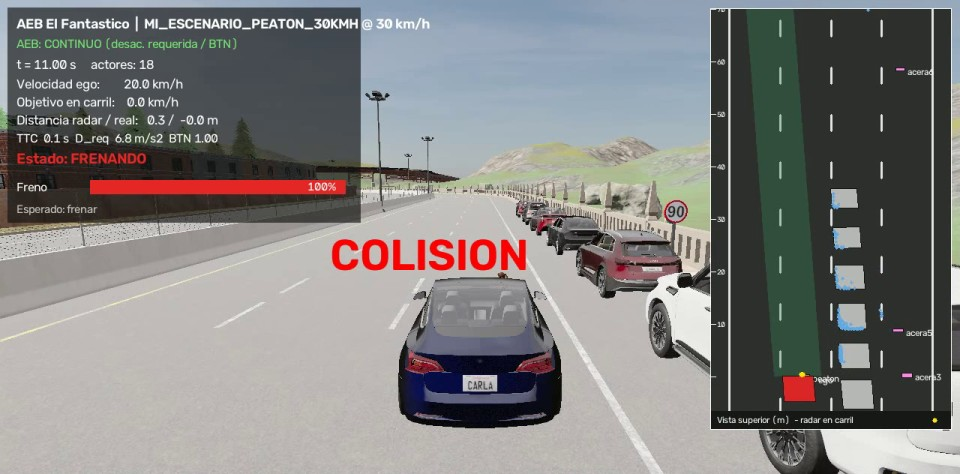
\includegraphics[width=\linewidth]{foto_nino_sin.jpg}\\
    \footnotesize (c)
  \end{minipage}
  \caption{Simulación en CARLA con el modelo del pedal: (a)
  \texttt{ENCAP\_CCRb\_6\_12} en $t=2.0$~s, estado FRENANDO con BTN${}=0.76$;
  (b) niño que cruza tarde con predicción de cruce, $t=10.2$~s, frenando a
  21.7~km/h; (c) misma situación sin predicción, impacto en $t=11.0$~s.}
  \label{fig:pedal_fotos}
\end{figure*}

\subsection{Observaciones}

Tres efectos de CARLA deben considerarse al interpretar estos resultados.
Primero, al soltar el acelerador el vehículo ya desacelera hasta
3.7~m/s$^2$ a 50~km/h; en CCRb, $b_C$ permaneció en cero hasta 2.0~s porque
esa desaceleración superaba a la objetivo, lo que oculta parte del retardo del
pedal (Fig.~\ref{fig:pedal_encap}a). Segundo, justo antes de detenerse, cerca
de 3~km/h, aparecen picos de unos 9~m/s$^2$ que no provienen del pedal.
Tercero, el tráfico de ambiente alteró el frenado final, con picos de unos
24~m/s$^2$, y aumentó la separación en CCRb de 1.31 a 2.34~m; por ello, las
mediciones se reportan sin tráfico. Por último, $p_{log}$ es un índice
geométrico del giro del pedal, no una presión hidráulica, y los parámetros
supuestos de la Tabla~\ref{tab:pedal_param} deben validarse en el banco de
pruebas.
\endgroup
